\subsection{Phase 2}
  We will then do the following post-processing steps:

  \begin{enumerate}
    \item Do flips isolating large botfans.
    \item treat long chains of $Z$'s
    \item handle the blue faces that are still large
  \end{enumerate}

  Before we start with these preprocessing steps let us define the blue faces as they are now as \emph{strips} that in some cases still have to be subdivided.

  \subsubsection{Phase 2.1}
    In every face we look for large (4 or more edges) topfans.

    \begin{invariants}
      \label{inv:uni:load}
      \item The edges on a fence obey the following $2$ loaded edges are followed by at least $1$ unloaded edge
    \end{invariants}

    For every sequence of large topfans not separated by large botfans we flip the following:
    1. Left rim of the first fan.
    2. The left rim of every further odd fan.
    3. The right rim of the last fan.

    In particular: For a large topfan not neighbored by any other large topfans we recolor both rims.

    Note that we only flip rims of a $T_+$.

    We do not flip the first and last edge we would normally flip in a strip. If this edge does not separate the large topfan from at least three top edges we dont flip these edges.

    \begin{lemma}
      \label{lm:uni:removingLargeB-fans}
      We create blue $(5, \infty)$-faces containing all the large topfans while obeying Invariant \ref{inv:uni:load}.
    \end{lemma}
    \begin{proof}
      TODO \fxwarning{TODO But easy by the above construction}
    \end{proof}

  \subsubsection{Phase 2.2}
    While doing this in a strip that (partially) lies above another face we can then create a chain of $Z$'s. We have two kinds of these chains with the same orientation and opposite orientation.

    See figure \ref{fig:uni:chains}

    \begin{figure}
      \centering
      \begin{subfigure}[b]{0.45 \textwidth}
          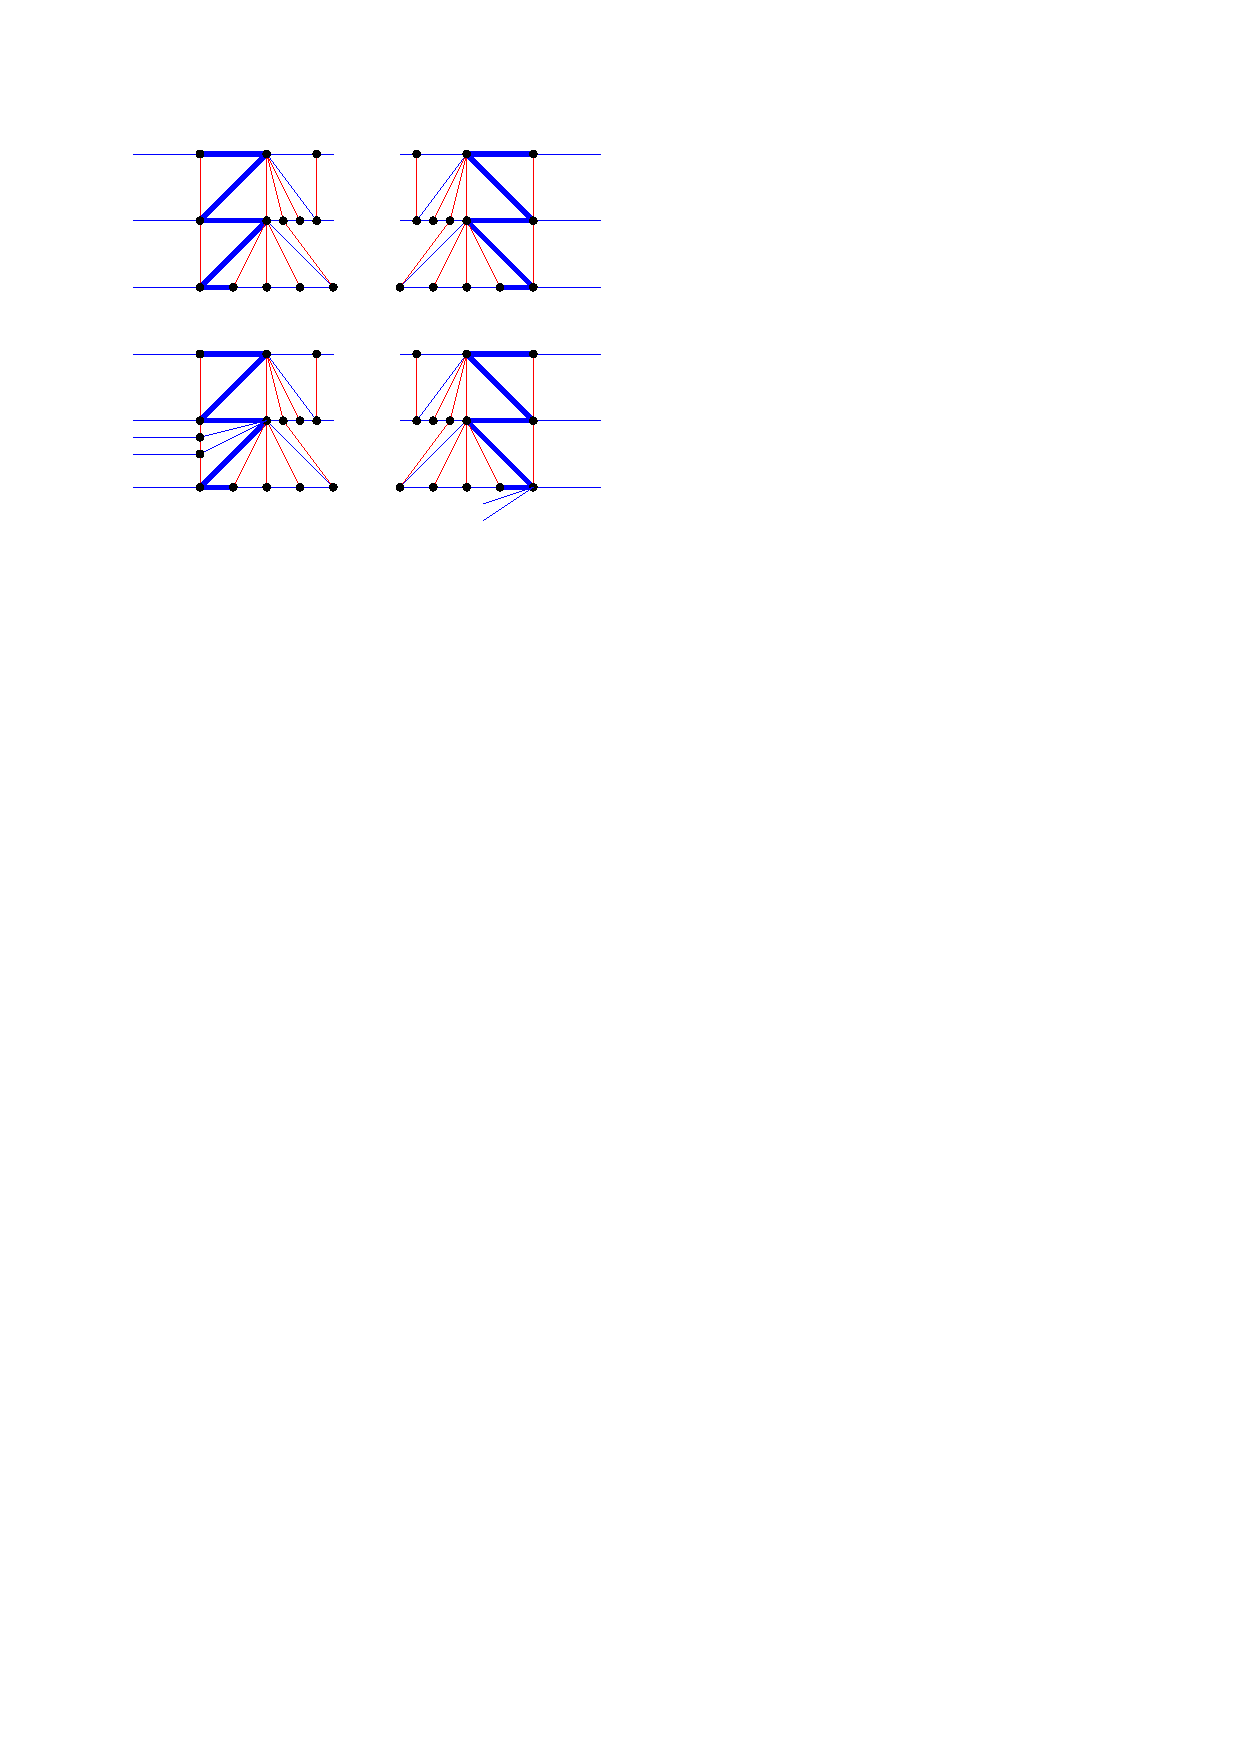
\includegraphics[width = \textwidth]{unifiedAlgo/img/post/sameChain}
          \caption{Same orientation}
      \end{subfigure}
      ~
      \begin{subfigure}[b]{0.45 \textwidth}
          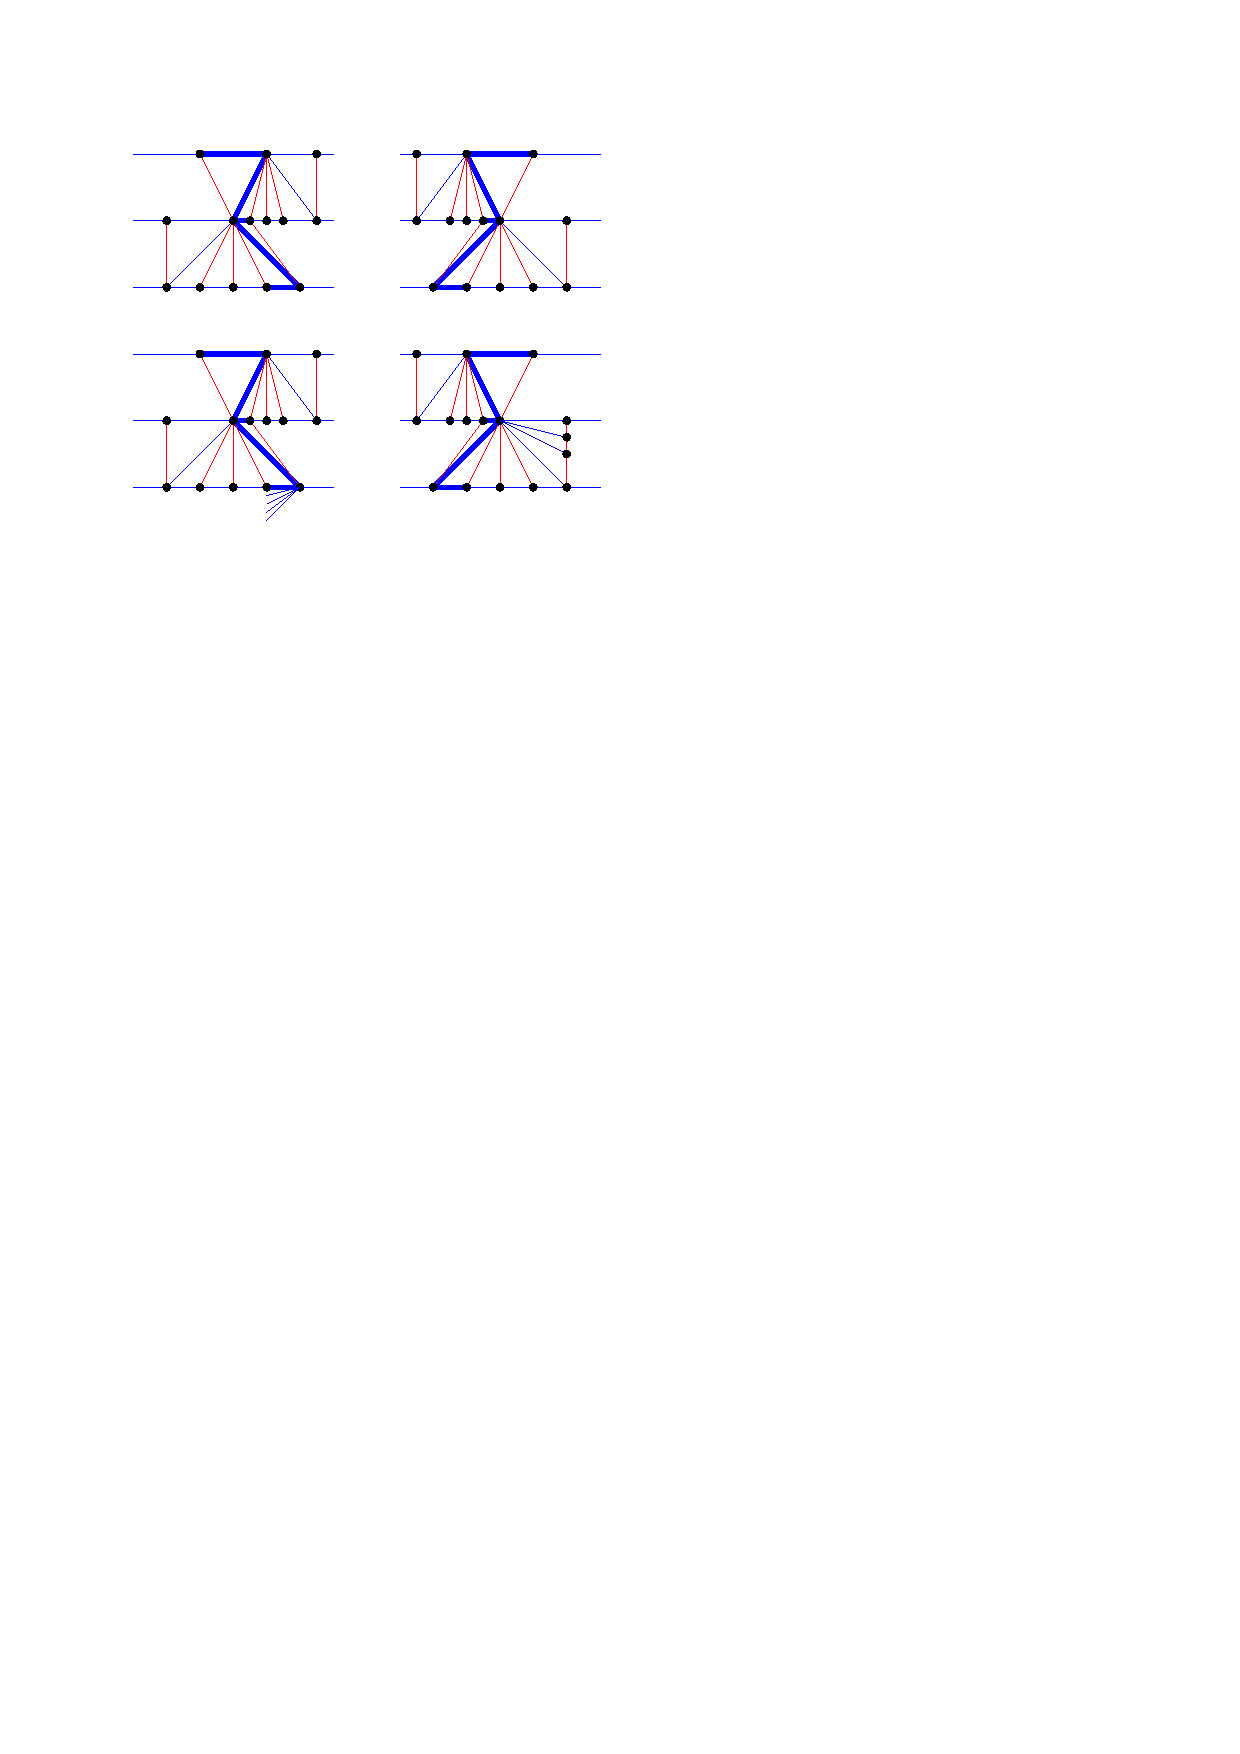
\includegraphics[width =\textwidth]{unifiedAlgo/img/post/oppChain}
          \caption{Opposite orientation}
      \end{subfigure}
      \caption{}
      \label{fig:uni:chains}
    \end{figure}

    From this phase we require the following.
    \begin{lemma}
      \label{lm:}
      After this phase all large topfans are in $9$-sided blue faces. All blue faces that are not $9$-sided consist of only $B$-fans and small $T$-fans.
    \end{lemma}

    \begin{proof}
      This follows from the way in which we entomb the large topfans.

      Clearly every large topfan is in a $9$-sided blue face. This even holds when we have a large topfan next to an opening and a closing of the face.
       \fxwarning{TODO small figure}

       By contraposition it is also clear that every face that is not $1$-sided cannot contain any large topfans and  thus consists of solely small topfans and botfans.
    \end{proof}

    We define a \emph{flip} as a series of changes to a REL turning it to another valid REL.
    We first do a flip turning every same orientation chain of $Z$'s to an opposite orientation one. Then we do a flip breaking an opposite orientation chain. We do this for every chain of $Z$'s created in Phase 2.1.

  We will work from the last created face upwards. When doing a flip we try to only alter the history, not the current face and certainly not the future. We will treat flips under a topfan of size 4 differently, because we do not have the space to execute all standard flips.

  \mypar{Size of left joints}
  We will show the following

  \begin{defi}
    A \emph{left joint} is the vertex in a $Z$ with at least two outgoing blue edges.
  \end{defi}

  A left joint corresponds with a split.

  \begin{lemma}
    \label{lm:}
    A left joint not adjacent to $\pS$ with a split has no top fan below it.
  \end{lemma}
  \begin{proof}
    If we are not adjacent to $\pS$ the only reasons for a split vertex $v_i$ are a chord or a polebound separating 2-chord.

    We will first consider the case of a chord.

    Let $v_i$ denote the split vertex. And $v_j$ denote the vertex where the path that split off joined the sweepcycle again (merge vertex). The chord that causes (the bottommost represent of) this split and merge is from $w_i$ to $w_j$ with $v_i$ connected to $w_i$ and $w_{i+1}$ and $v_j$ to $w_j$ and $w_{j-1}$ (cf. chord and chord multi figures). (See description of evading a chord irregularity).

    Now in the next candidate walk $w_i$ and $w_j$ are next to each other and both have a $B$-fan of size at least $2$ (to $v_i$ and $w_{i+1}$ and to $v_j$ and $w_{j-1}$ respectively.)

  \end{proof}

  \mypar{The standard flips}
  Figures of the basic same and opposite orientation flips.
   See Figure \ref{fig:uni:sameFlip}, \ref{fig:uni:sameFlipComplete} and \ref{fig:uni:oppFlip}.

  \mypar{Flips under a topfan of size 4}
  Suppose we have a topfan $F$ of size $4$
  As long as there is only one chain of $Z$'s with one of the rims of $F$. We can just execute a regular flip without running out of space.




  \mypar{Same orientation flip}

  In this case we do the flip in Figure \ref{fig:uni:sameFlip}

  \begin{figure}[h]
    \centering
    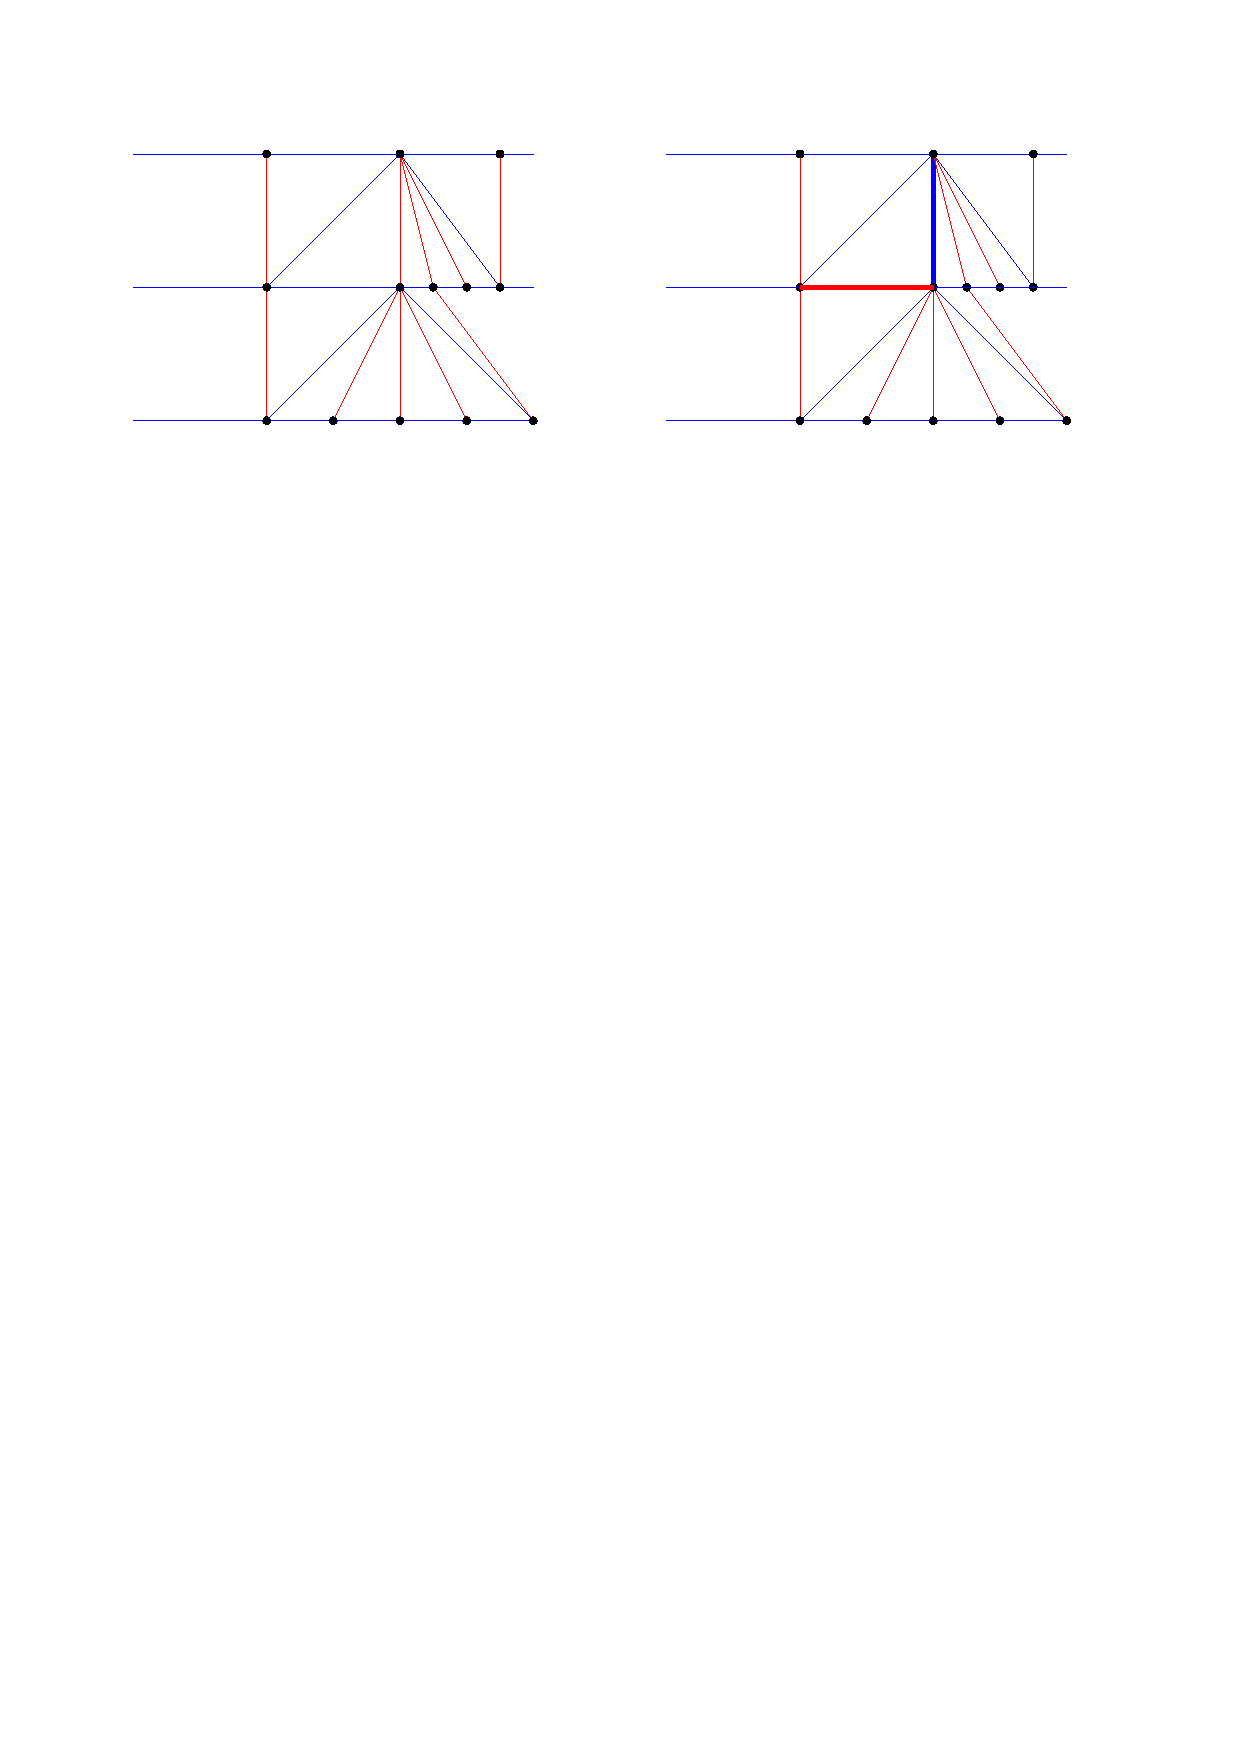
\includegraphics[width =\textwidth]{unifiedAlgo/img/post/sameFlip}
    \caption{The flip we execute on same direction chains}
    \label{fig:uni:sameFlip}
  \end{figure}

  \begin{figure}[h]
    \centering
    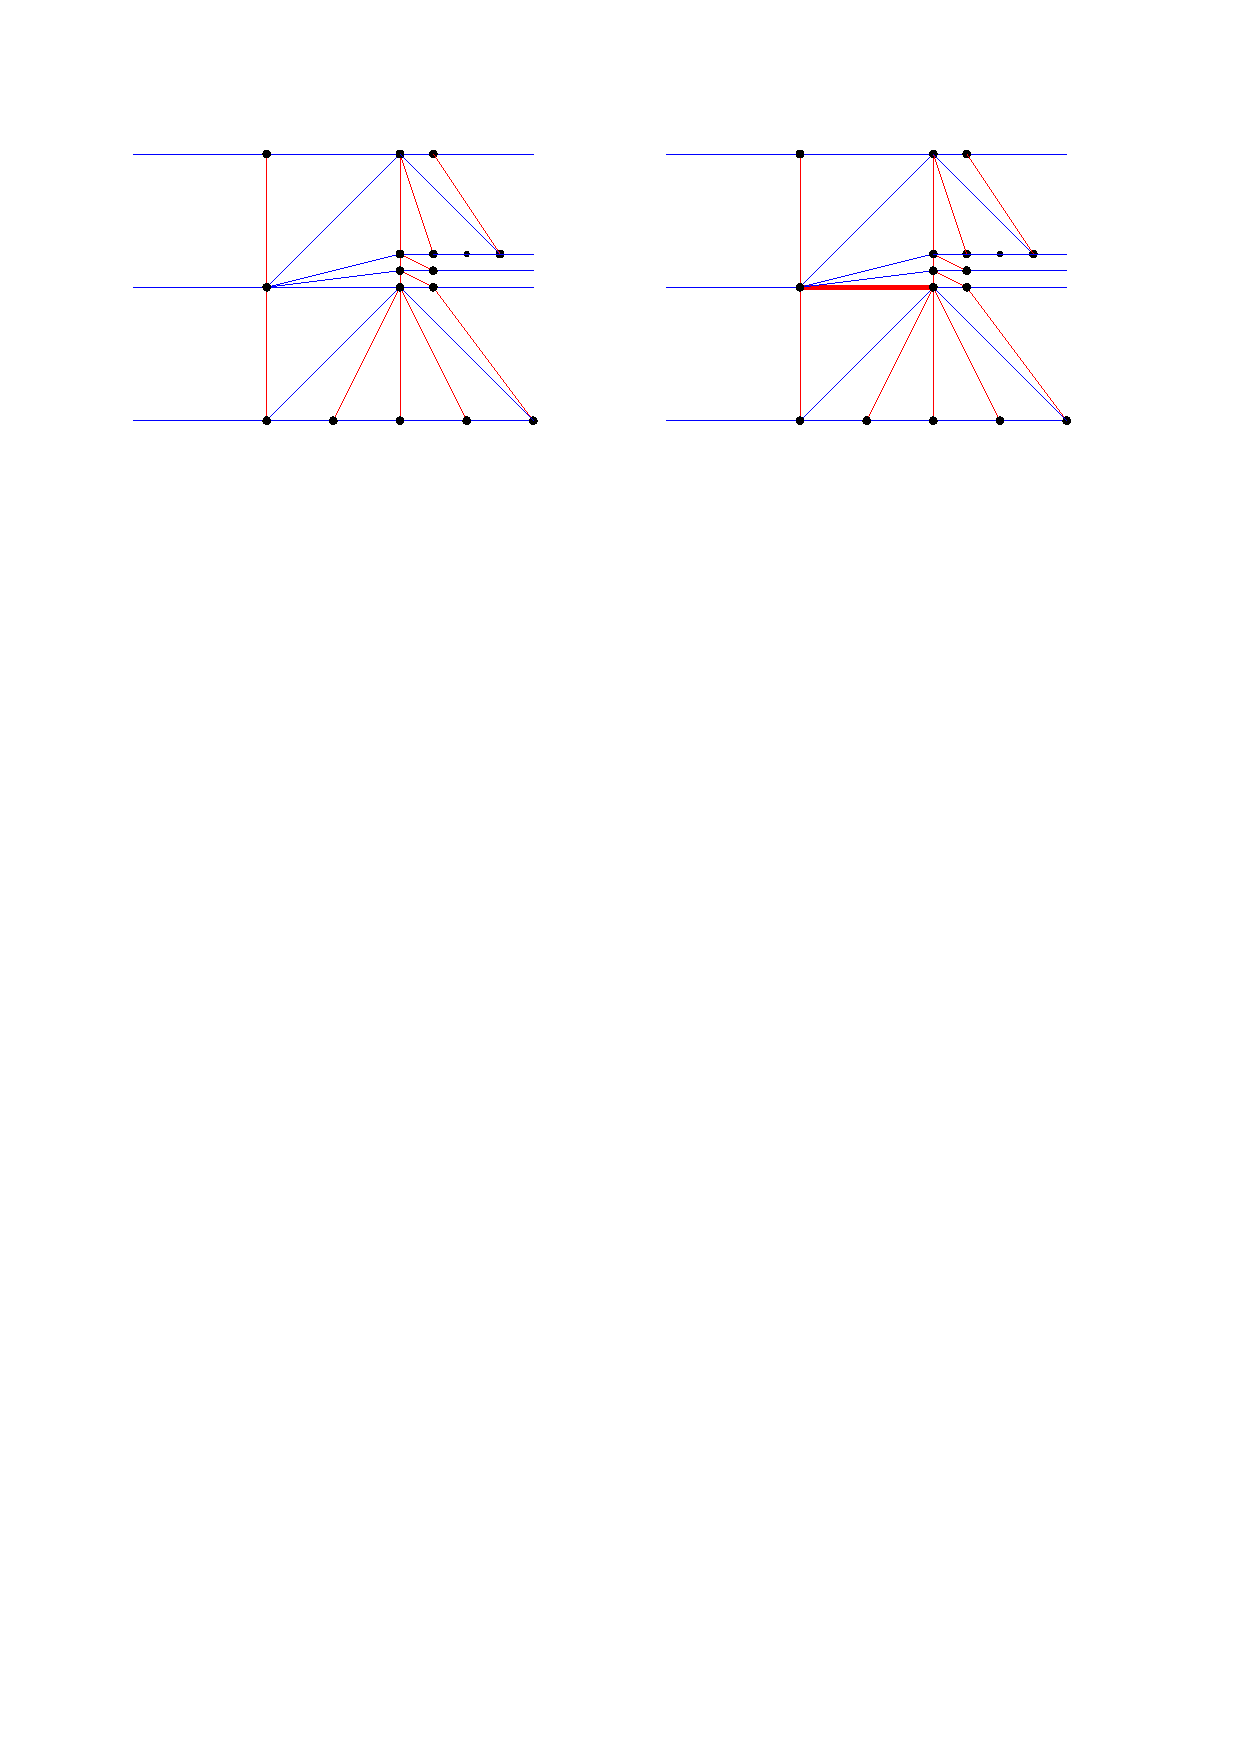
\includegraphics[width =\textwidth]{unifiedAlgo/img/post/sameMultiFlip}
    \caption{The flip we execute on same direction chains with multiple edges in the middle joint}
    \label{fig:uni:sameMultiFlip}
  \end{figure}

   after this flip we changed the chain and now we have a chain of oppositely oriented $Z$'s. Luckily we know how to treat these. See Figure \ref{fig:uni:sameFlipComplete}.

   \begin{figure}[h]
     \centering
     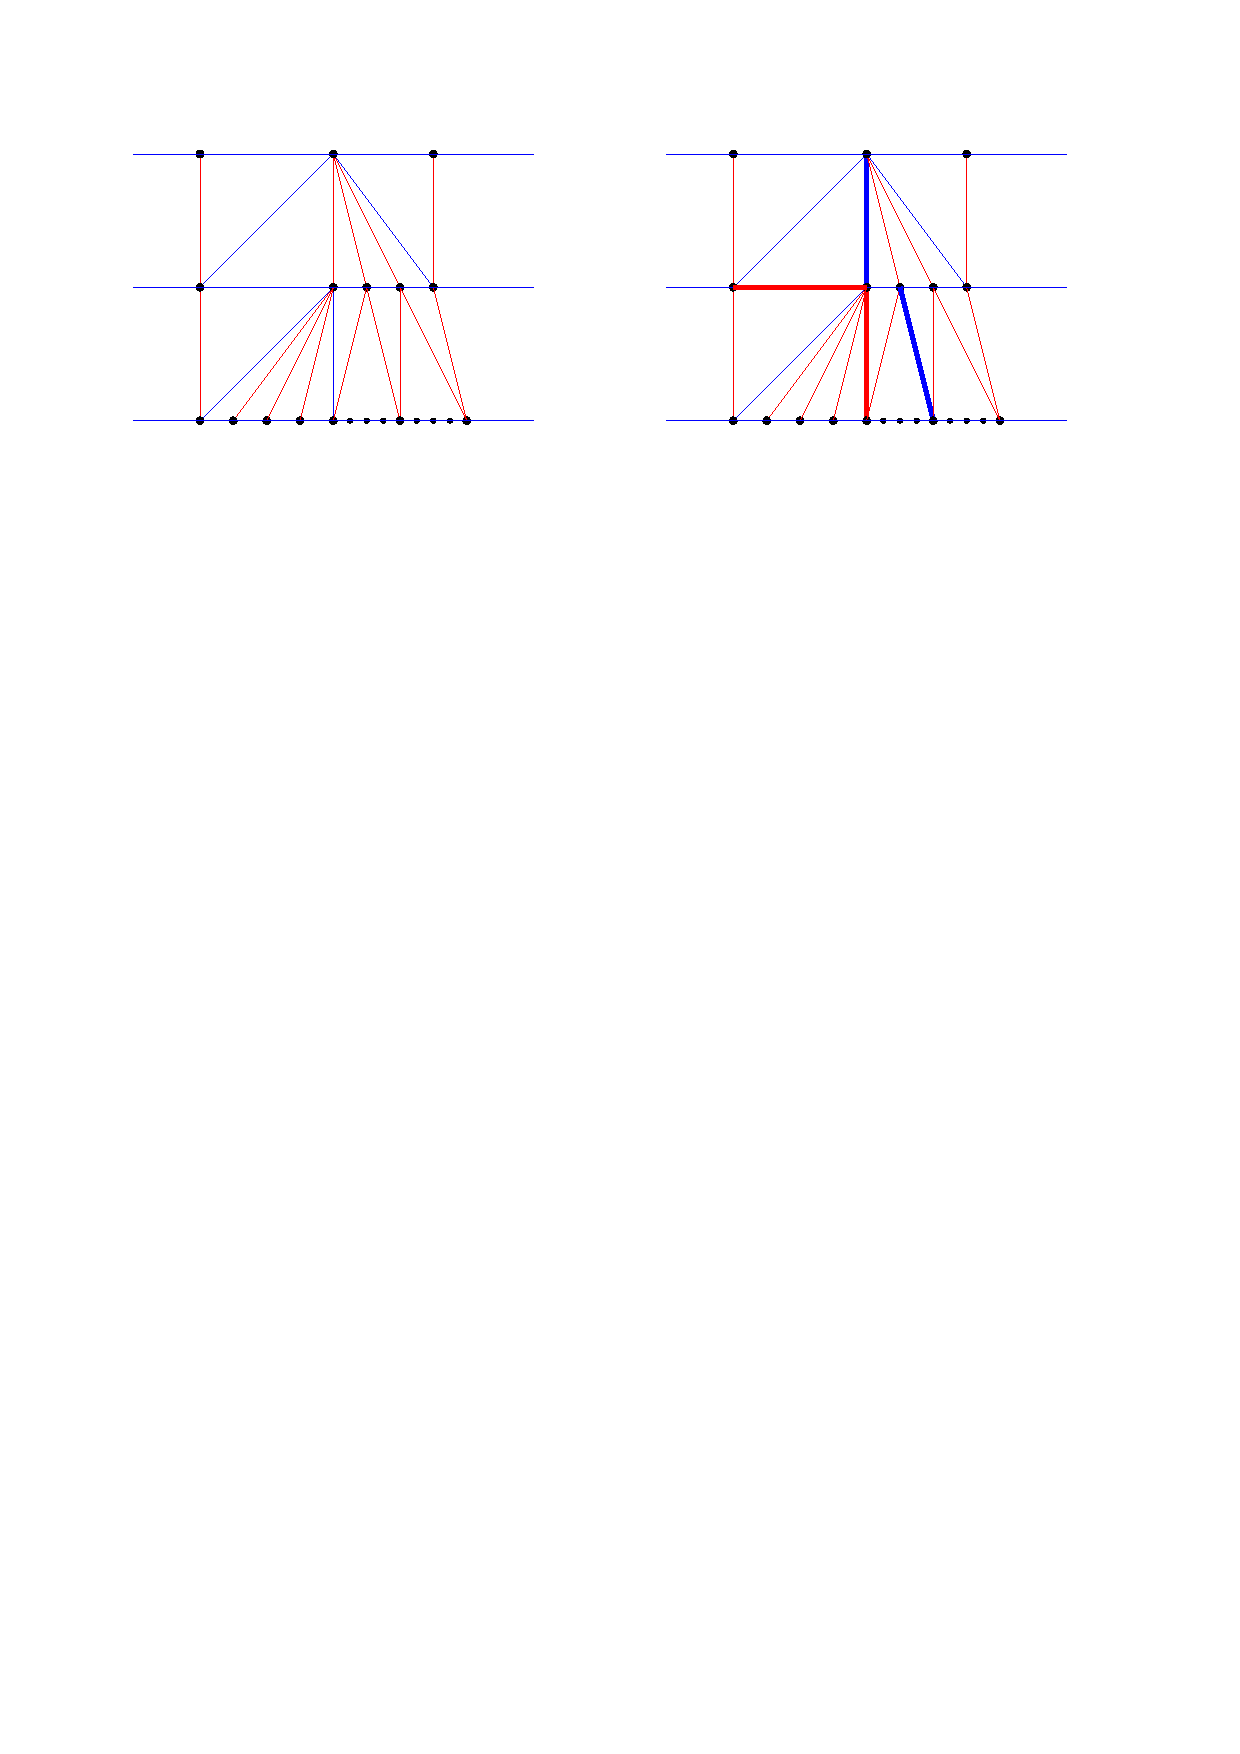
\includegraphics[width =\textwidth]{unifiedAlgo/img/post/sameFlipComplete}
     \caption{The result of both flips}
     \label{fig:uni:sameFlipComplete}
   \end{figure}

   \fxwarning{TODO This flip in a multi case}
   \fxwarning{TODO Argue why these edges are like they are}


   \mypar{Opposite orientation flips}
   We namely execute the flip given in Figure \ref{fig:uni:oppFlip}. The small vertices on the bottom-left hint on the possibility of vertices but those do not have to be there.

  \begin{figure}[h]
    \centering
    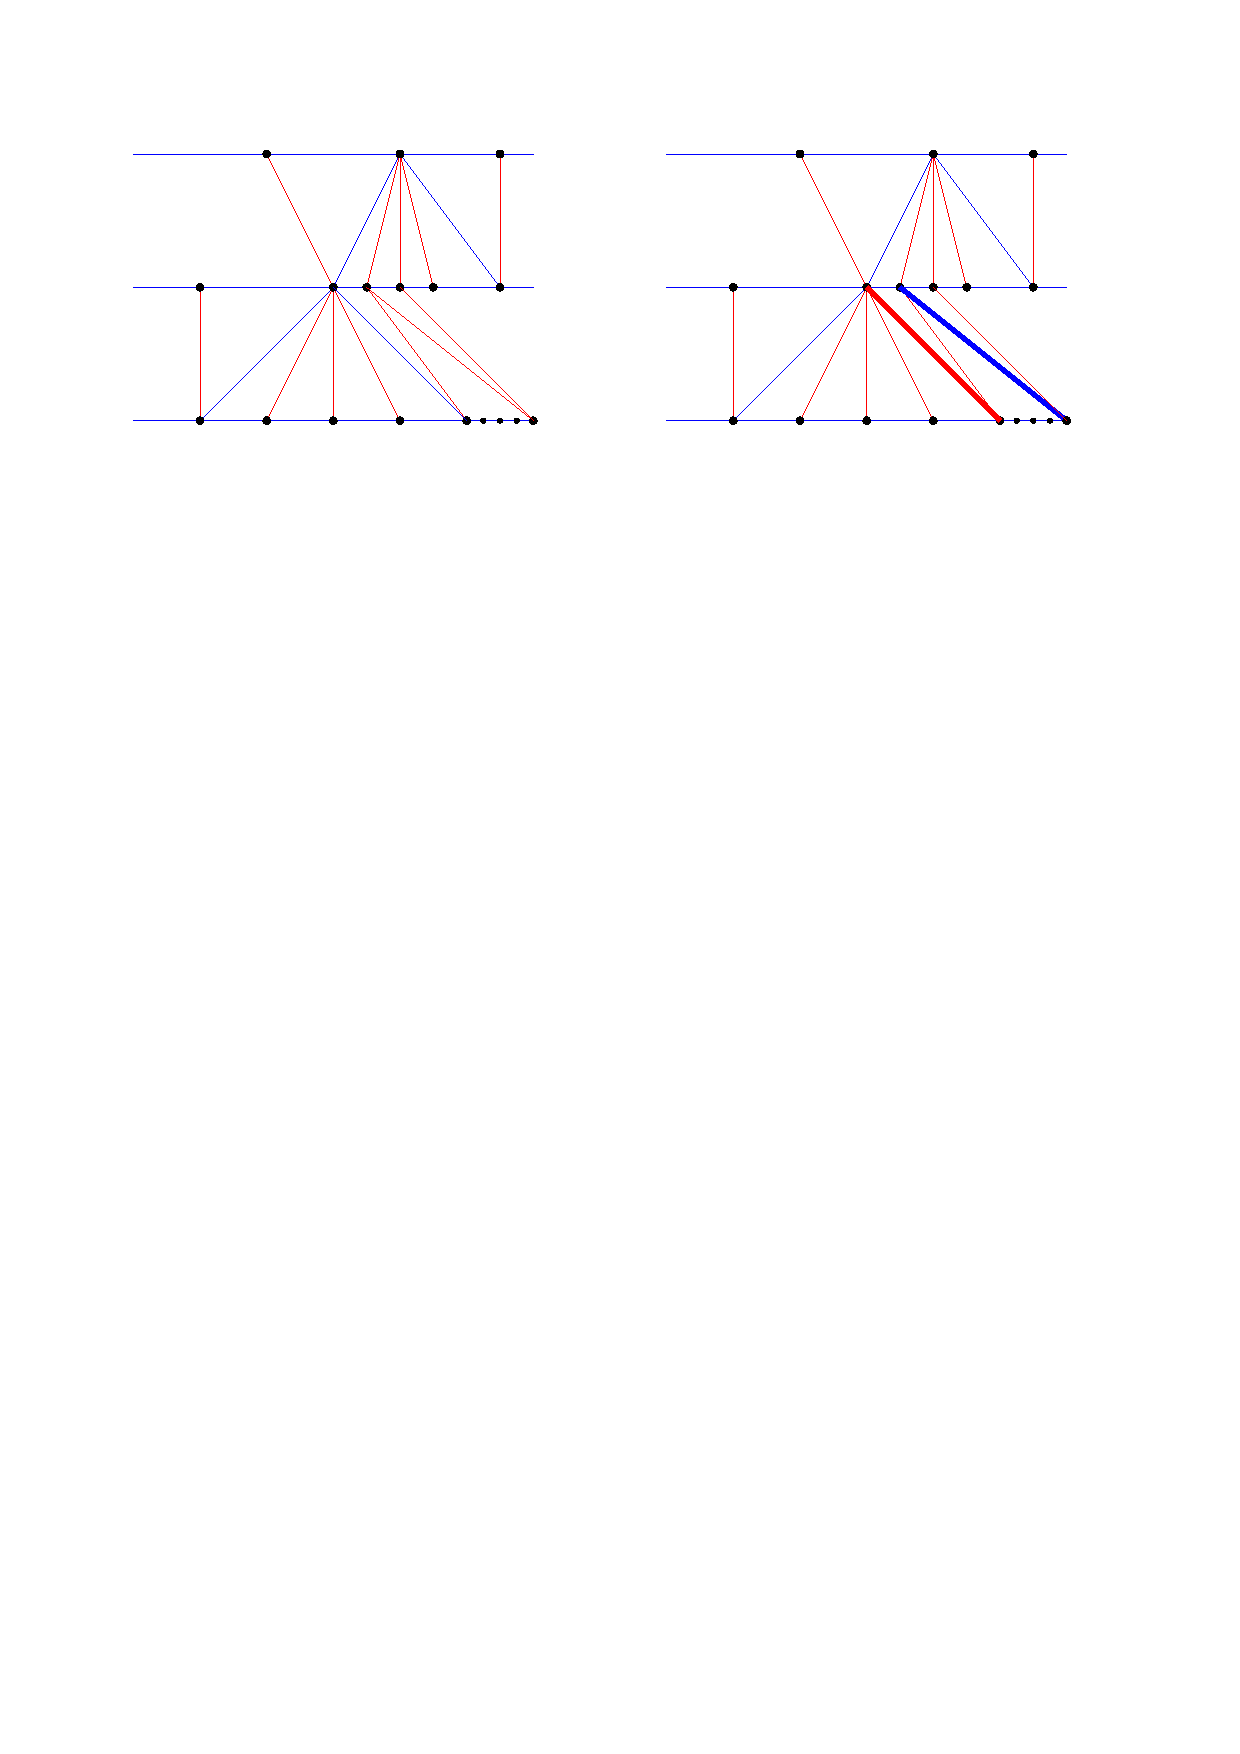
\includegraphics[width = \textwidth]{unifiedAlgo/img/post/oppFlip}
    \caption{The flip we execute on opposite chains}
    \label{fig:uni:oppFlip}
  \end{figure}

  \begin{figure}[h]
    \centering
    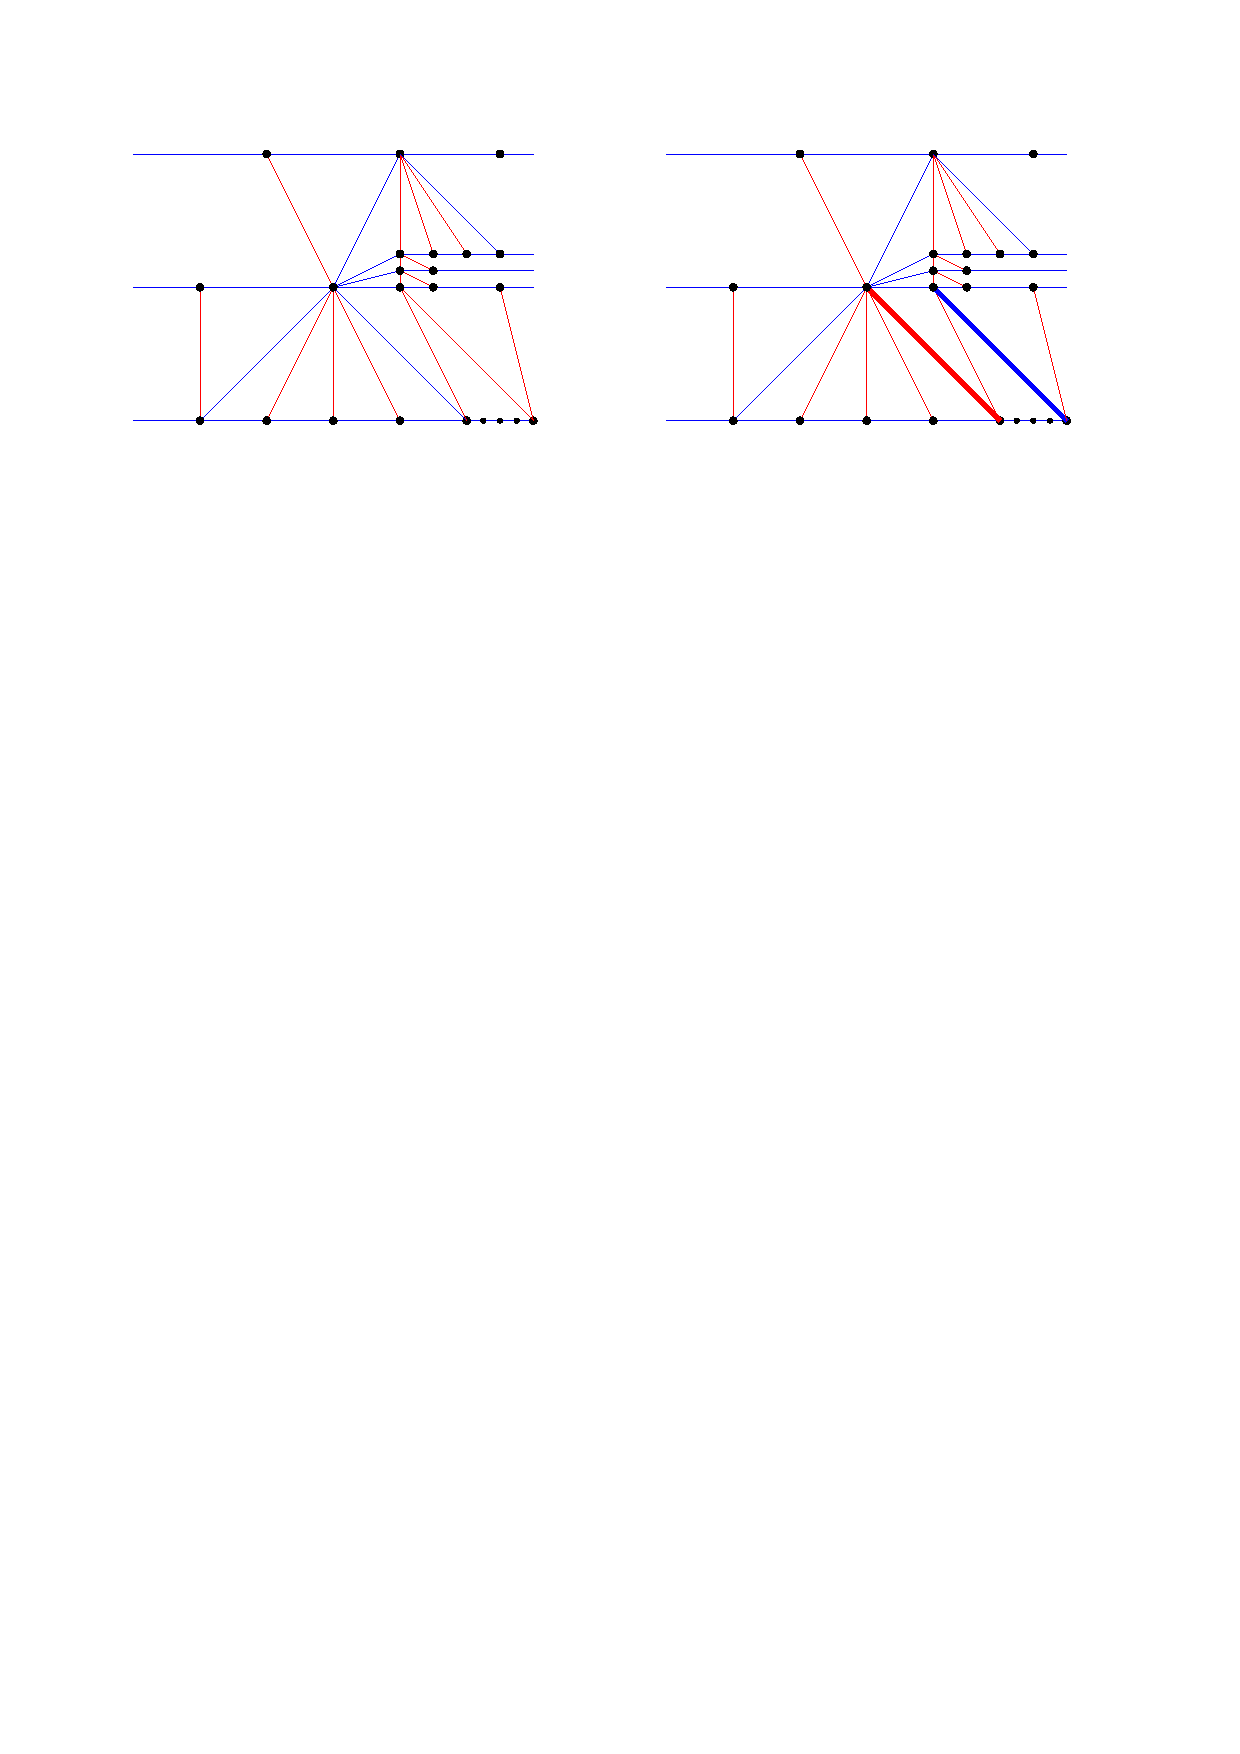
\includegraphics[width = \textwidth]{unifiedAlgo/img/post/oppMultiFlip}
    \caption{The flip we execute on opposite chains with multiple edges in the middle}
    \label{fig:uni:oppMultiFlip}
  \end{figure}

  When recoloring the edge blue in this flip it might be above another $Z$ and thus create a chain of $2$ $Z$'s. However this chain can grow no further as above this newly blue edge there is a red closing triangle.

  \fxwarning{TODO this flip in a multi case}
  \fxwarning{TODO Argue why these edges are like they are}


  \mypar{Flips with multiple edges in the middle joint.}


  We will want to proof the following about these flips.

  \begin{lemma}
    \label{lm:}
    Faces in already treated strips will never grow with more than $2$ on the top. In particular faces containing a large topfan will remain 3-sided. At the same time there will be no more chains of more then $2$ $Z$'s.
  \end{lemma}

  \begin{proof}
    Let us first describe the effects of both flips.

    We apply a flip when in the current face we discover that we have 2 subsequent $Z$'s. Then applying the flip we change the size of faces in the history. \fxnote{And it will make talking of strips more difficult since we reshape them and not only subdivide them.}

    Let us first describe how these flips change the faces in the historic strips.
    \fxwarning{TODO but first I will describe flips on $Z$'s with a middle fan}
    \begin{figure}[h]
      \centering
      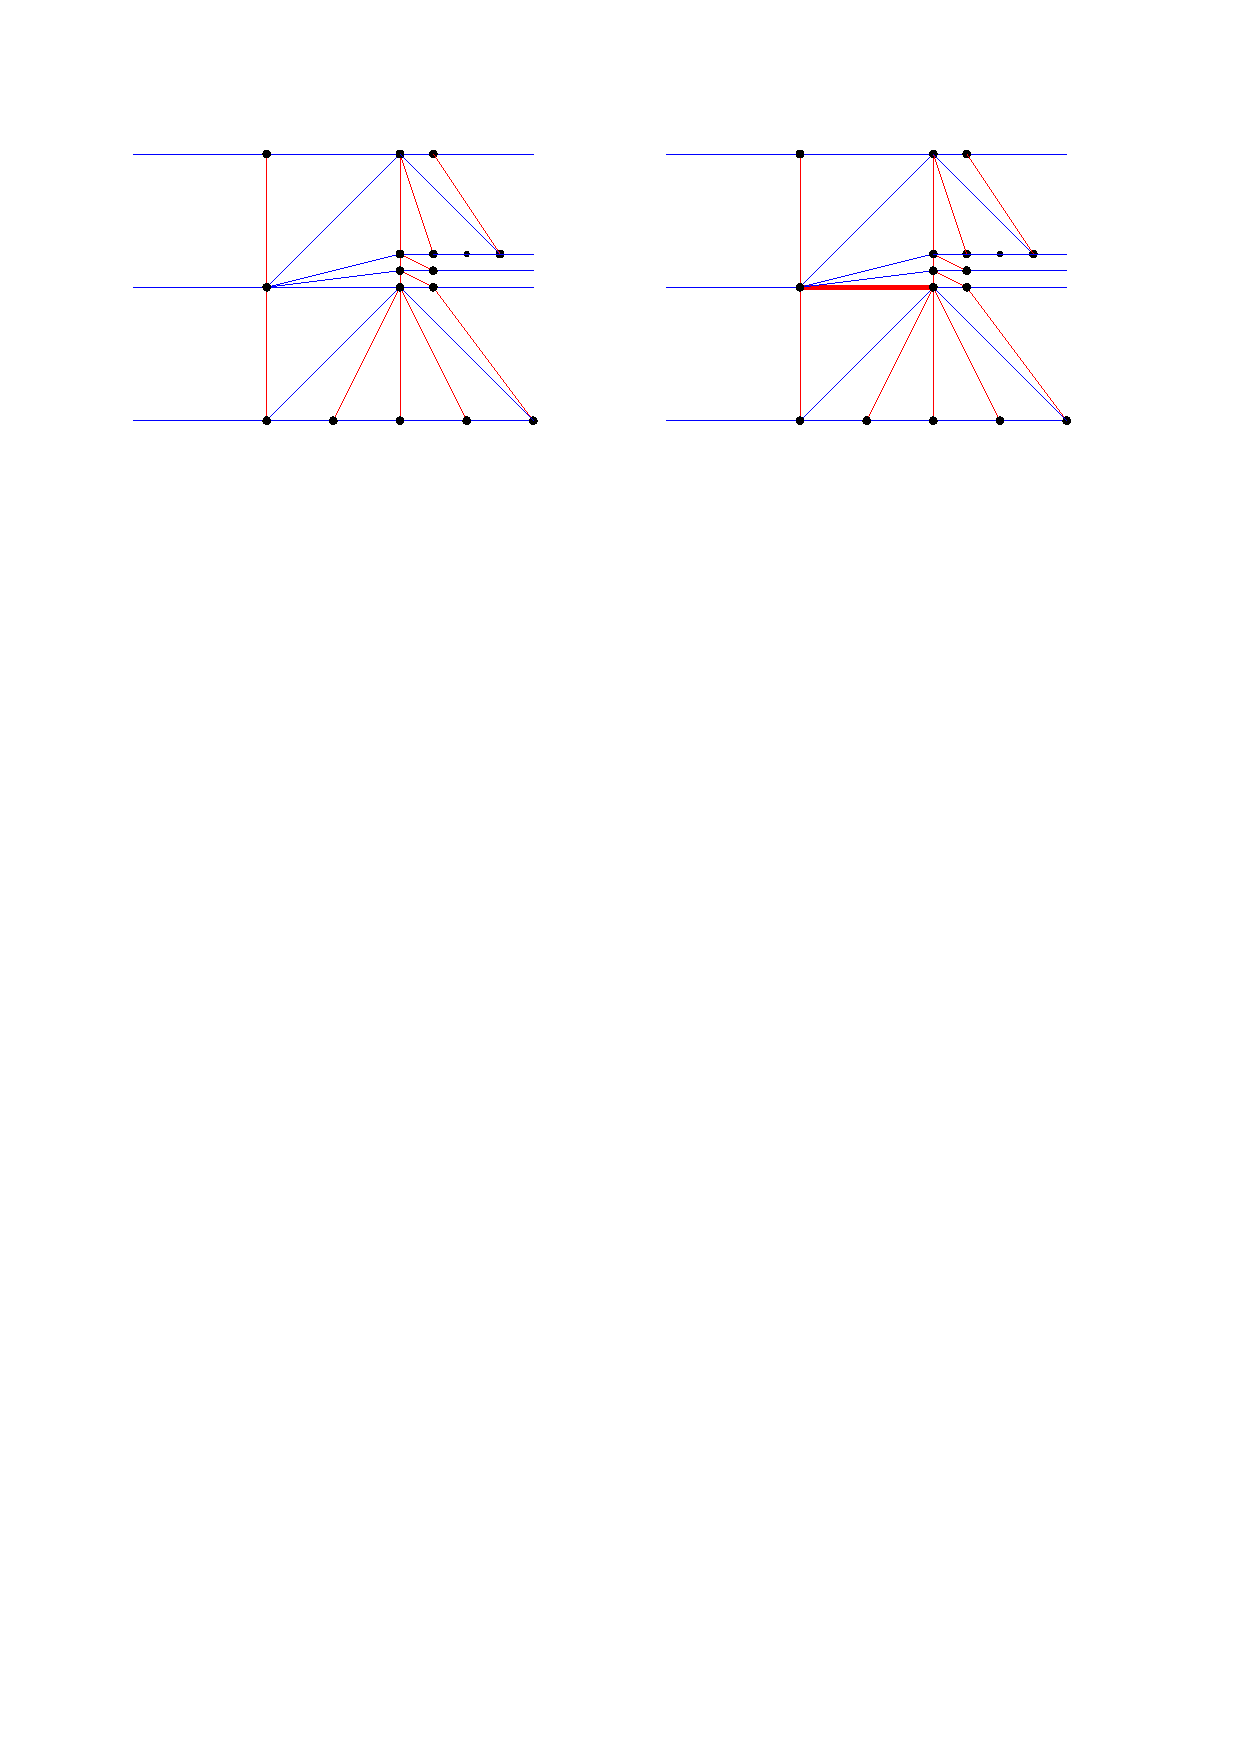
\includegraphics[width =\textwidth]{unifiedAlgo/img/post/sameMultiFlip}
      \caption{The flip we execute on same direction chains with multiple edges in the middle joint}
      \label{fig:uni:sameMultiFlip}
    \end{figure}
    The same orientation flip lengthens one historical face by one vertex on the top and one on the bottom. While the multiflip connects two faces, but will not create a large topfan \fxnote{or maybe one larger. We can definitely connect large topfans this way}.

    The opposite orientation flip follows the same orientation flip without middle edges. And this case it makes one historic face 1-1 longer and another historic face 1-1 shorter. If the shortened face becomes to short we drop this edge.
    The face we elongate now is a different face from the one we elongated in the previous flip.

    Furthermore if we only have to do an opposite chain flip then we simply elongate a face by $1-\infty$ and shorten another face by $1-\infty$. Again we drop the shortened face if it becomes to short (i.e. less then $1-1$)

    \mypar{Every face is only hit a number of times}
    *Once on each side during same direction flips
    *Once during opp flips (per side)

    OR

    * Just once

    OR

    * We just do not care as long as we do not open topfans (Hint: we do not)
    * However we do enlarge topfans (at most by 1 on every side) so we end up with $3-\infty$ topfans.

    Every two subsequent $Z$'s are treated in one flip. This flip makes a historic faces longer but closes them in such a way they can not be opened by other flips.

    \mypar{Remaining $Z$'s}
    The opp flip can place an blue edge above another blue edge. However this chain stops here since above this is a red split vertex. So the longest chain of $Z$'s is now of length two.
  \end{proof}
